% !TeX root = ../tfg.tex
% !TeX encoding = utf8

\chapter{Marco experimental y metodología}
\label{chapter:methodology}

Como se ha podido observar en el \autoref{chapter:tda}, el TDA proporciona una
serie de mecanismos que nos permiten estudiar con bastante fidelidad la
topología de los datos en CNNs. Además, hemos visto que dichas redes tienden a
simplificar la forma de los datos durante su paso a través de las distintas
capas y lo hacen de manera diferente en función de la arquitectura propuesta. En
este capítulo se describe la metodología así como las herramientas empleadas para
analizar distintas CNNs en profundidad.
%En este capítulo, aplicaremos el TDA para estudiar a fondo cómo afectan las distintas componentes y mecanismos comúnmente empleados en el entrenamiento de las CNNs en el marco de la topología. Además, trataremos de analizar cómo afecta la topología de los datos a la capacidad de generalización de los modelos y a su transferencia de conocimiento. Nuestra hipótesis en base a los estudios previamente citados apuntan a que una complejidad topológica menor en las etapas finales del modelos podrían mejorar su rendimiento en clasificación, mientras que una complejidad mayor podría facilitar la transferencia de conocimiento.

\section{Experimentos}

Los experimentos se han dividido en tres etapas con el fin de comprender cómo
las CNNs transforman la topología de los datos. Para ello, se han entrenado una
serie de modelos pertenecientes a tres familias de arquitecturas diferentes de
CNNs: ResNet-18, DenseNet-121 y EfficientNet-B0. El principal motivo para seleccionar
estos representantes y no alternativas más complejas de la misma familia se debe
a que an mostrado una buena capacidad de generalización y eficiencia.

La \textbf{primera etapa} ha consistido en la comparación de la complejidad
topológica de los datos a lo largo de la red en función de la arquitectura, el tamaño
de lote y el optimizador escogido.% Para ello, se han evaluado los tamaños de lote 8, 16, 32 y 64 y los optimizadores SGD y Adam.

En la \textbf{segunda etapa}, se ha escogido el mejor modelo para cada una de
las dos granularidades del conjunto de datos tratado y se ha comparado la
topología de los datos con los mismos modelos entrenados con aumento de datos, la
granuralidad del conjunto de datos y la partición de datos.

En la \textbf{última etapa}, se han realizado dos experimentos en base a las observaciones
realizadas en las anteriores etapas. Como veremos en la
\autoref{sec:homology-analysis}, nuestra hipótesis en base a los estudios realizados
apuntan a que una complejidad topológica relativa menor en las etapas finales del
modelos podrían mejorar su rendimiento en clasificación, mientras que una
complejidad mayor podría facilitar la transferencia de conocimiento a conjuntos
de datos más complejos. Por ello, se propone tratar de mejorar la clasificación
del modelo mediante el uso del regularizador topológico descrito en la
\autoref{subsec:regularizer}.

\section{Entorno de experimentación}

Para la realización de este proyecto se seleccionó Python como lenguaje de programación
principal, dada su amplia disponibilidad de herramientas de análisis de datos
\cite{10.5555/1593511}. En particular, se utilizó la versión 3.10.14 por su compatibilidad
con una variedad de bibliotecas importantes para la investigación realizada.
Para la gestión del entorno de desarrollo se empleó Anaconda \cite{anaconda}, facilitando
así la configuración reproducible de los entornos de trabajo. El código
implementado puede consultarse en el repositorio de GitHub
\href{https://github.com/pab1s/tda-nn-analysis}{\texttt{tda-nn-analysis}}\footnote{https://github.com/pab1s/tda-nn-analysis}.

Los modelos de aprendizaje profundo se implementaron utilizando PyTorch 1.13.1
\cite{NEURIPS2019_9015}, una biblioteca de cálculo tensorial que soporta la aceleración
por GPU. PyTorch es conocido por su extensiva colección de herramientas que
simplifican el desarrollo de modelos de aprendizaje profundo, siendo ampliamente
reconocido y utilizado en la investigación en inteligencia artificial.

El análisis de homología persistente se llevó a cabo mediante la biblioteca \texttt{giotto-tda}
0.6.0 \cite{giotto-tda}, que se apoya en \texttt{ripser} \cite{ctralie2018ripser}
por su eficiencia en la ejecución y el uso de memoria en comparación con otras opciones
disponibles \cite{Otter_2017}. Además, esta herramienta permite el procesamiento
multihilo, lo que es un beneficio adicional importante. Para completar los experimentos,
se empleó el paquete \texttt{torch\_topological}\footnote{\href{https://pytorch-topological.readthedocs.io/en/latest/}{https://pytorch-topological.readthedocs.io/en/latest/}}
0.1.7, que implementa el cálculo de la homología persistente de la filtración de
Vietoris-Rips de forma que sea compatible con la retropropagación en PyTorch. %se utilizó \texttt{scikit-learn} 1.5.0 para la implementación del algoritmo de LLE.

Para la visualización de datos, se optó principalmente por \texttt{matplotlib} 3.8.4
\cite{hunter2007matplotlib} y \texttt{seaborn} 0.13.2
\cite{michael_waskom_2017_883859}, herramientas que ofrecen funcionalidades avanzadas
para la creación de gráficos y visualizaciones complejas. También se usó \texttt{torch-cam}
0.4.0 \cite{torcham2020} para la visualización de las activaciones en la imagen.
Adicionalmente, se integraron bibliotecas auxiliares como \texttt{pandas} 2.2.2
\cite{mckinney2010data} y \texttt{numpy} 1.26.4 \cite{2020NumPy-Array} para
cálculos numéricos adicionales\footnote{Una lista completa de paquetes y
	requisitos se encuentra disponible en el archivo
	\href{https://github.com/pab1s/tda-nn-analysis/blob/main/environment.yaml}{\texttt{environment.yaml}}
	en el repositorio del proyecto.}.

Los experimentos se realizaron en el \textit{switch} Dionisio de la partición
Dios del clúster de servidores GPU ubicado en el edificio CPD Santa Lucía de la
Universidad de Granada, perteneciente al Instituto Andaluz Interuniversitario en
\textit{Data Science and Computational Intelligence}\footnote{\href{https://dasci.es/}{https://dasci.es/}}
(DASCI). Está equipado con dos CPUs Intel Xeon Silver 4216 @ 2.10GHz, 512 Gb de
RAM y dos GPUs Quadro RTX 8000 con 48Gb de VRAM.

\section{Conjunto de datos}

Durante el desarrollo de los experimentos se ha empleado una versión modificada del
conjunto de datos \textbf{\textit{Vehicle Identification}}\footnote{\href{https://dasci.es/es/transferencia/open-data/vehicleid-es/}{https://dasci.es/es/transferencia/open-data/vehicleid-es/}}
publicado por el DASCI. Este conjunto de datos está compuesto de imágenes
frontales de coches en primer plano proveniente de diversas fuentes. El interés de
este conjunto de datos en particular radica en la su disposición de \textbf{distintas
	granularidades}. Es decir, disponemos de distintas clasificaciones en función de
lo \enquote{fina} que sea nuestra predicción sobre los detalles de los datos.
Esta versión se divide en dos conjuntos en función de su especificidad:

\begin{itemize}
	\item \textbf{Especificidad Marca}: consiste en 3232 imágenes etiquetadas en 34
	clases que indican la marca del fabricante del vehículo.
	
	\item \textbf{Especificidad Marca-Modelo}: consiste en 2701 imágenes etiquetadas
	en 152 clases identificando la marca y el modelo concreto del vehículo.
\end{itemize}

El principal motivo por el que se ha seleccionado este conjunto de datos es por su
disposición en las dos especificidades propuestas. Dado que las instancias son
comunes en la mayoría de los casos, resultará de gran interés saber cómo clasificar
conjuntos de datos prácticamente idénticos con distintas etiquetas puede afectar
al proceso de generalización y a la topología de los datos.

\begin{figure}[h]
	\centering
	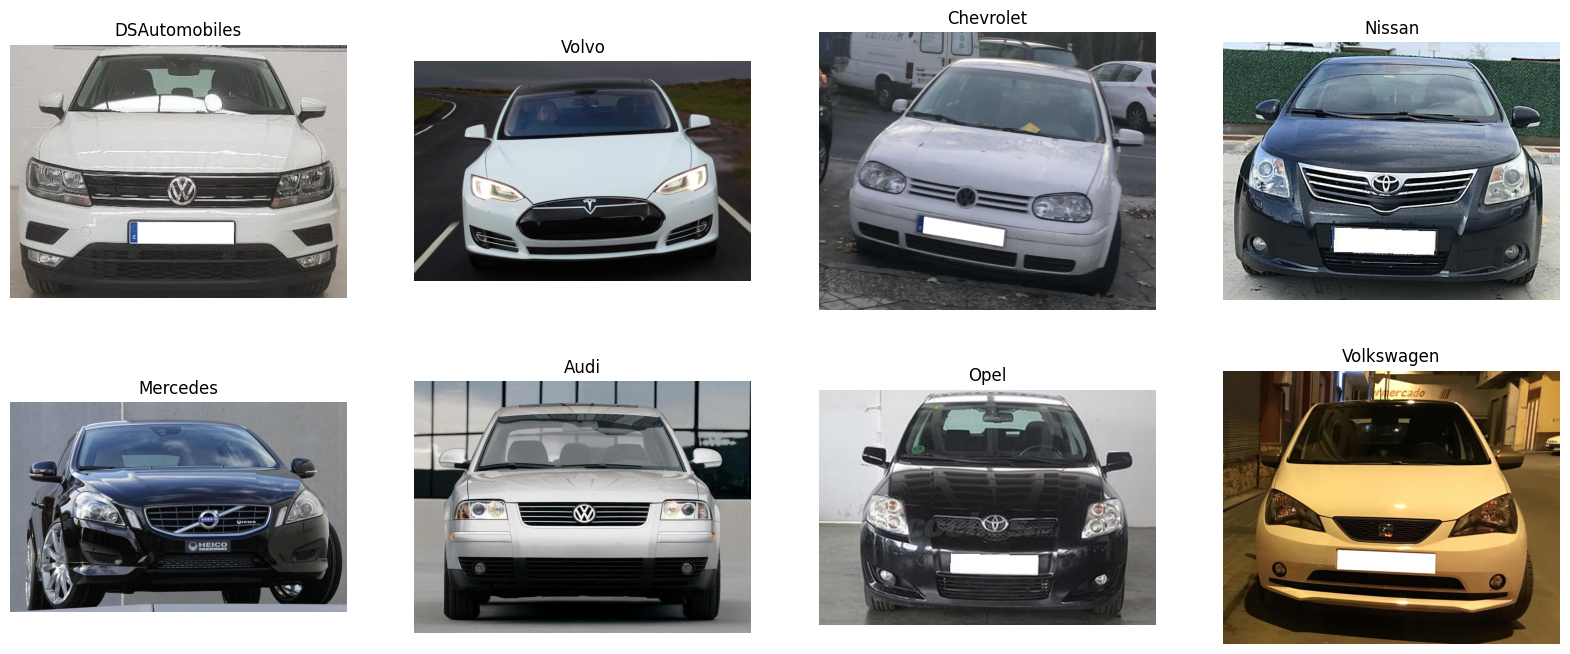
\includegraphics[width=120mm]{img/marca-example.png}
	\caption{Ejemplos de instancias por clase en la especificidad de Marca.}
	\label{fig:example-m}
\end{figure}

\begin{figure}[h]
	\centering
	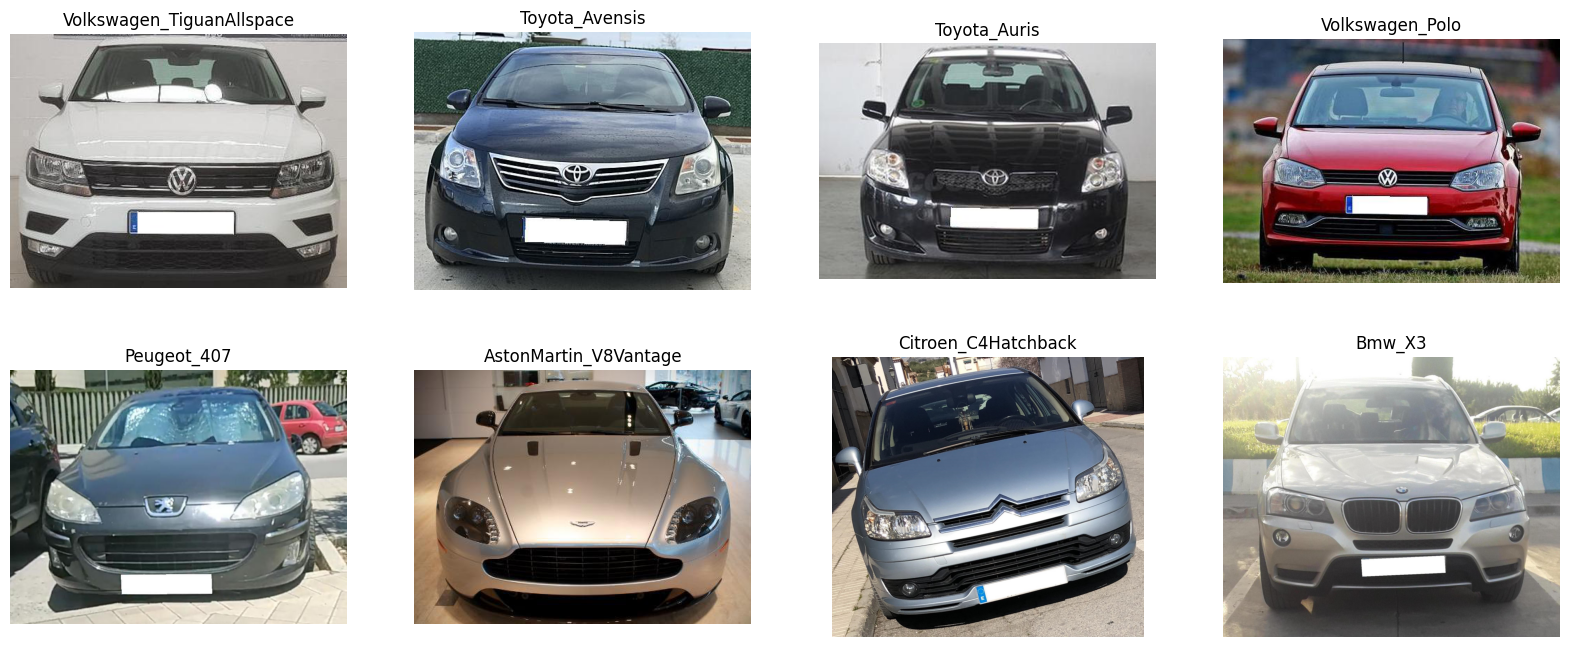
\includegraphics[width=120mm]{img/marca-modelo-example.png}
	\caption{Ejemplos de instancias por clase en la especificidad de Marca-Modelo.}
	\label{fig:example-mm}
\end{figure}

La \autoref{fig:imb-m} muestra un claro desbalance entre las distintas clases ambos
conjuntos de datos. De hecho podemos observar que en ciertas ocasiones el número
de muestras por clase es tan solo de una instancia, mientras que otras clases están
claramente sobrerrepresentadas.

\begin{figure}[h]
	\centering
	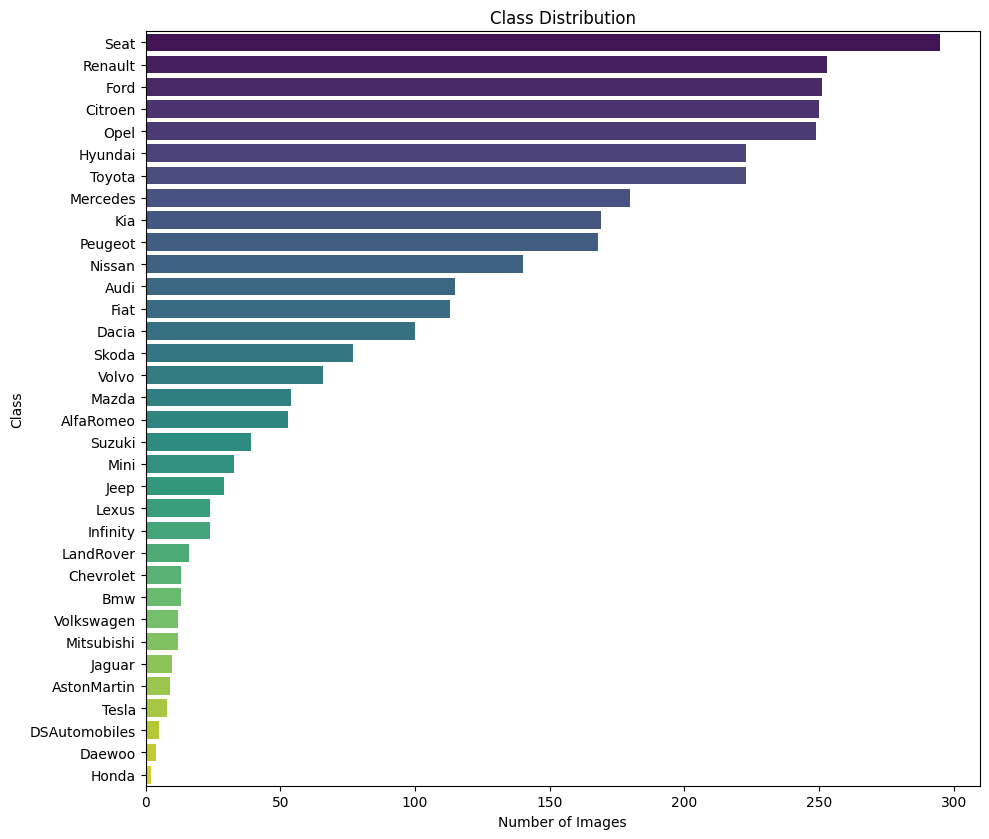
\includegraphics[width=100mm]{img/imbalance-marca.png}
	\caption{Número de instancias por clase en la especificidad de Marca.}
	\label{fig:imb-m}
\end{figure}

Este problema es aún peor cuando nos fijamos en la especificidad Marca-Modelo, tal
y como muestra la \autoref{fig:imb-mm}. Por este motivo, será interesante emplear
métricas cuya sensibilidad respecto a clases desbalanceadas sea mayor.

\begin{figure}
	\centering
	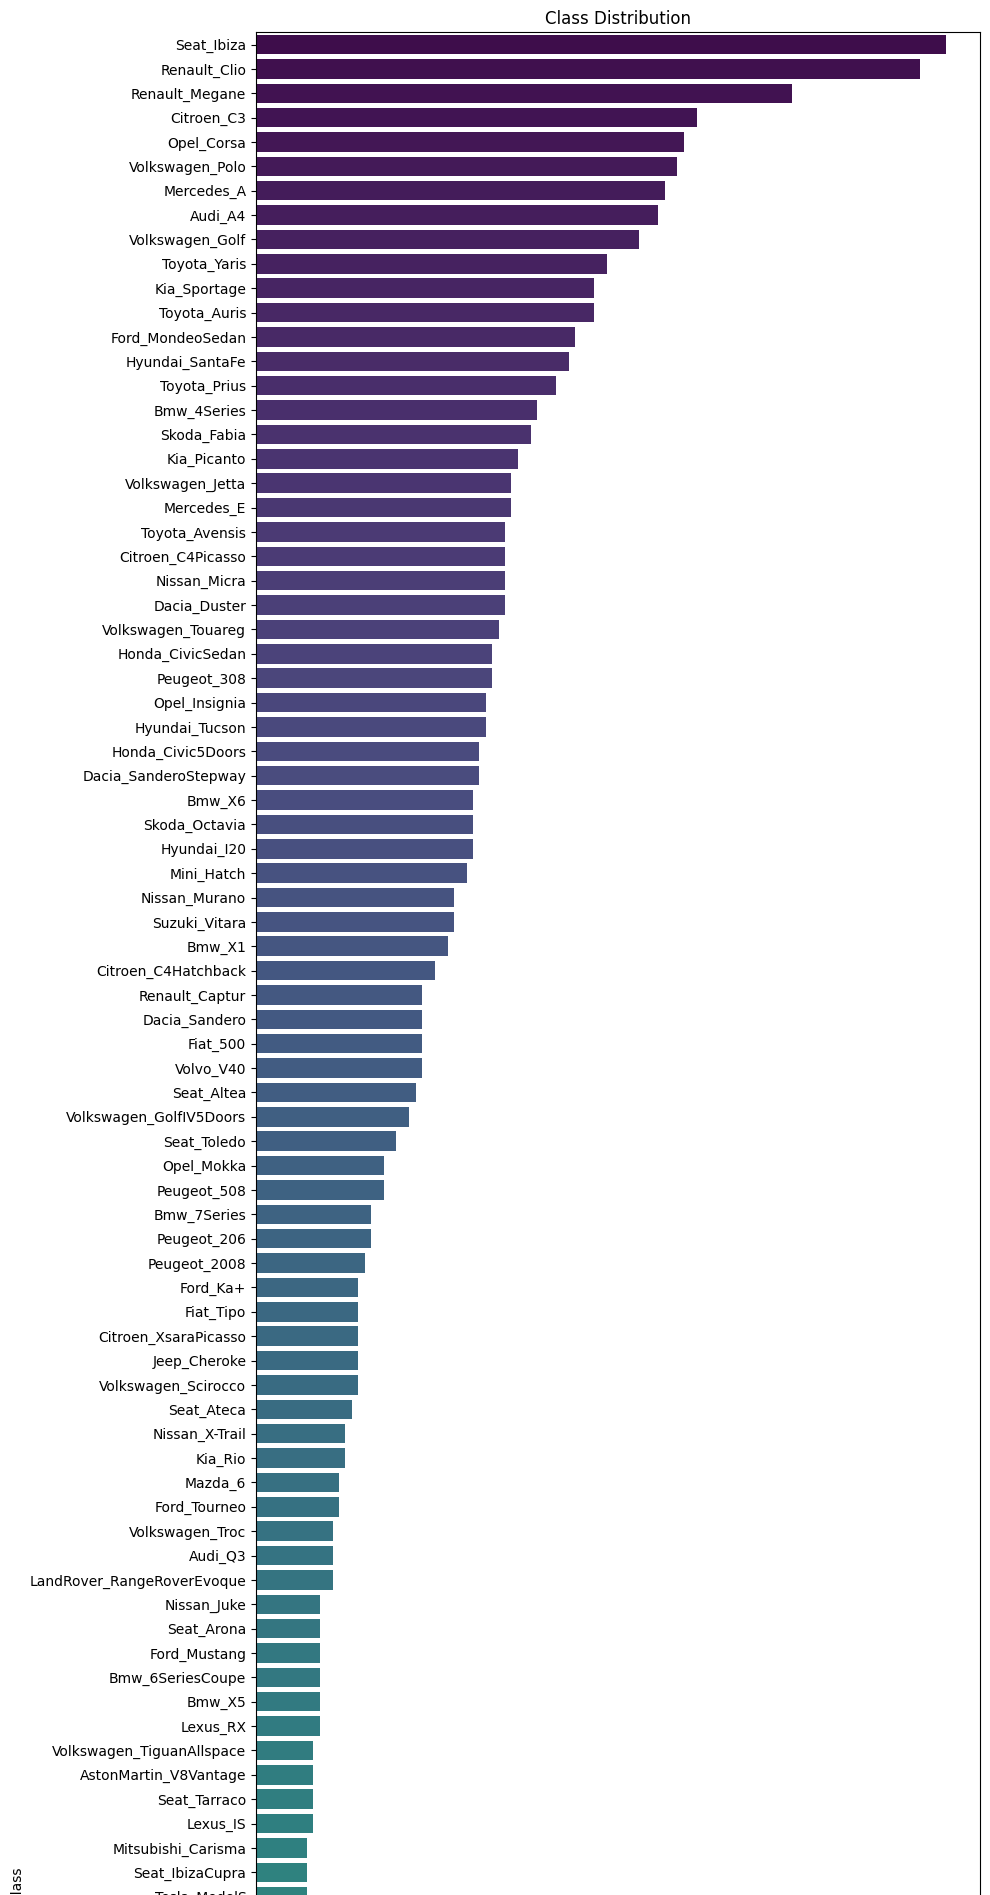
\includegraphics[width=110mm]{img/imbalance-marca-modelo-1.png}
\end{figure}

\begin{figure}
	\centering
	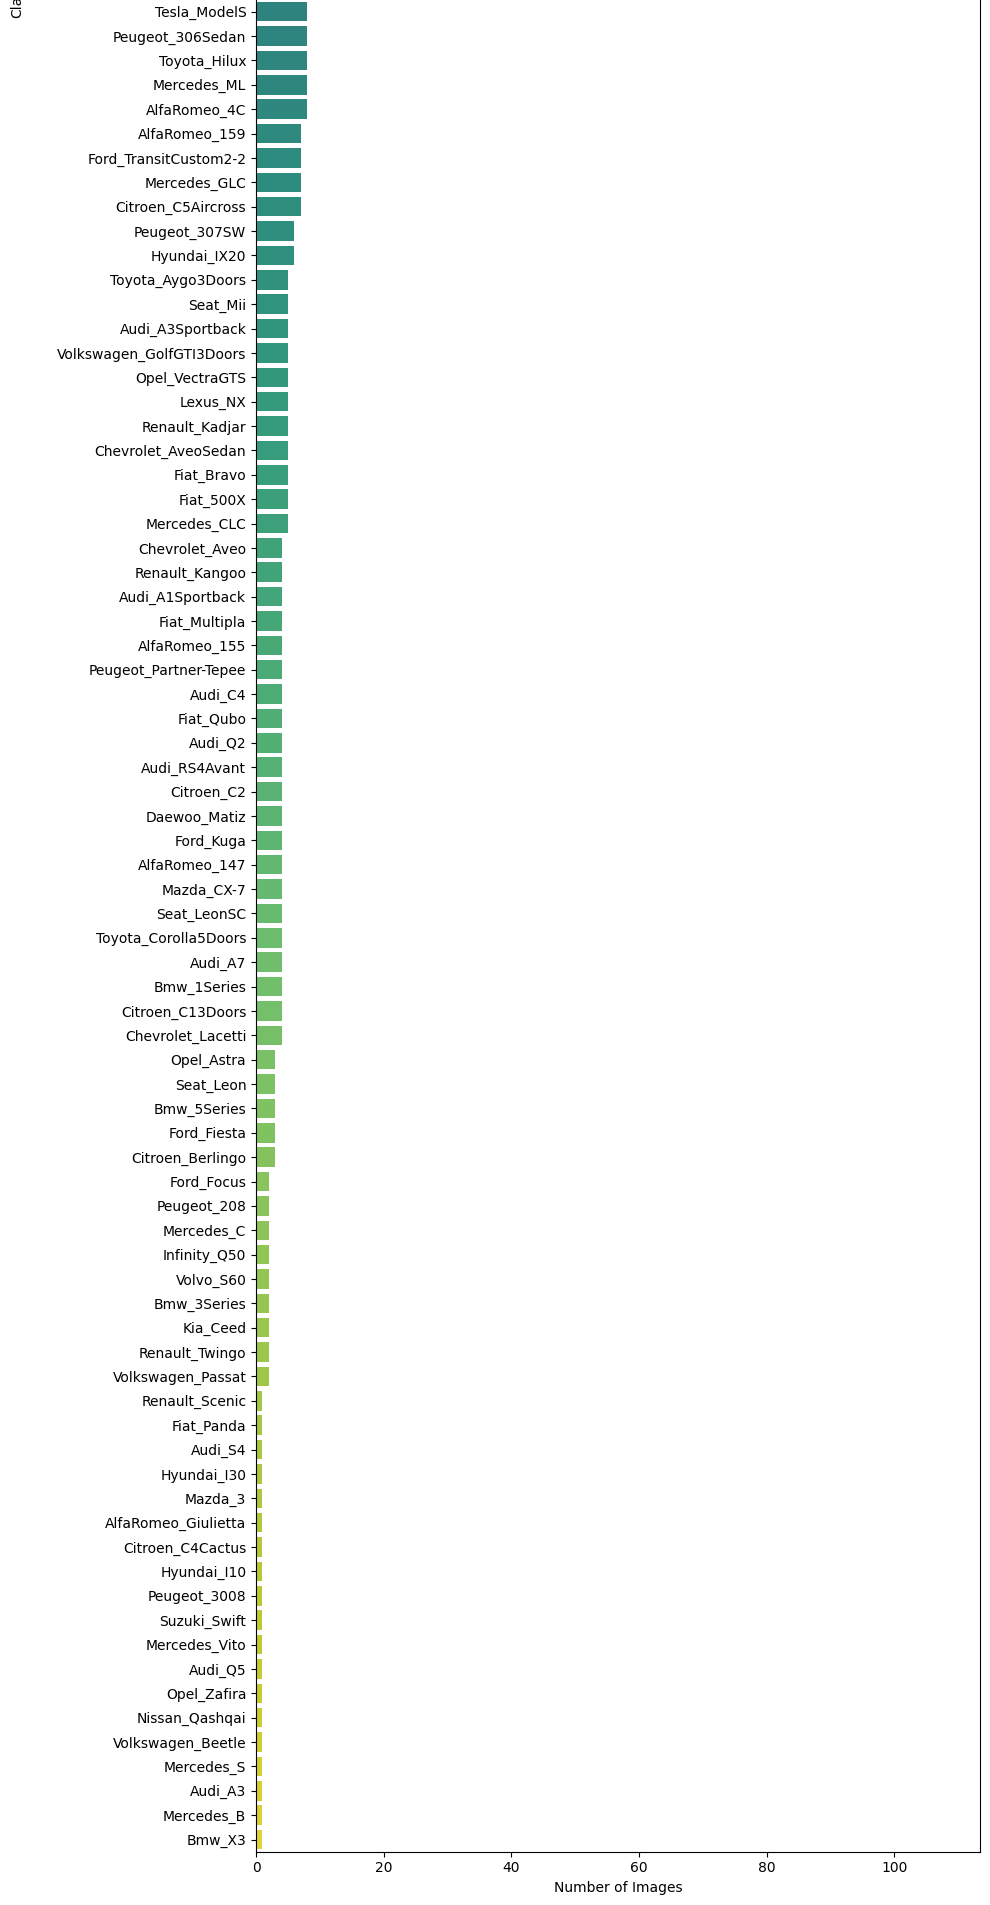
\includegraphics[width=110mm]{img/imbalance-marca-modelo-2.png}
	\caption{Número de instancias por clase en la especificidad de Marca-Modelo.}
	\label{fig:imb-mm}
\end{figure}

Ambos \textit{datasets} se dividirán en conjuntos de entrenamiento, validación y
test con una distribución 80-10-10 respectivamente durante el proceso de experimentación.
El conjunto de entrenamiento se empleará para ajustar los pesos de los modelos
directamente de las instancias que lo componen. El conjunto de validación se empleará
durante el proceso de entrenamiento para obtener una evaluación no sesgada de los
modelos con el objetivo de evitar el sobreajuste y mejorar su capacidad de generalización.
Finalmente, emplearemos el conjunto de test para obtener una evaluación final de
los modelos entrenados. Es importante destacar la importancia y diferencia de
estos dos últimos conjuntos de datos. Si bien ambos se emplean para evaluar los modelos,
prescindir del conjunto de validación para emplear también el de test supondría
un caso de \textbf{\textit{data snooping}} \cite{white2000reality}. Esto
significa que nuestros resultados finales se verían sesgados de manera indirecta
por las decisiones tomadas sobre las evaluaciones del conjunto de test, de forma
que nuestros resultados también estarían sesgados y nuestras conclusiones sobre la
generalización de los modelos serían incorrectas.

En un inicio, se valoró la posibilidad de realizar una validación cruzada para
comparar los resultados de las redes entrenadas. No obstante, dado que nuestro
objetivo es estudiar la topología de los datos en estas CNNs respecto a los
conjuntos de datos que disponemos y no necesariamente obtener el mejor modelo
posible, se descartó dicha opción. Además, el gran coste computacional del entrenamiento
de estos modelos, junto a los numerosos entrenamientos realizados, reforzaron esta
postura. Este enfoque permite centrar los recursos computacionales en el
análisis de la topología de los datos y la realización de los experimentos.

\section{Preprocesamiento de datos}
\label{sec:data-aug}

Dada la naturaleza heterogénea de las imágenes empleadas, todas las imágenes se
han redimensionado a $224 \times 224$ con un total de $3$ canales normalizado en
un rango entre $[0,1]$ para los colores RGB. Al estar los modelos preentrenados con
ImageNet, los colores de las imágenes se han tipificado respecto a la media y
desviación típica de dicho conjunto. Esto es, una media
$\mu = (0.485, 0.456, 0.406)$ y una desviación típica
$\sigma = (0.229, 0.224, 0.225)$.

Para los modelos entrenados empleando aumento de datos, se han estudiado las siguientes
transformaciones:

\begin{itemize}
	\item \textbf{Fluctuación del color}: aplica alteraciones en el brillo,
	contraste y saturación base de las imágenes. Dada una imagen, se modifica
	cada uno de estos valores $\alpha$ en un factor obtenido de una distribución
	uniforme $\mathcal{U}([u, v])$, siendo $u = \max\{0, 1 - \alpha\}$ y $v = 1 +
	\alpha$.
	
	\item \textbf{Desenfoque Gaussiano}: se desenfoca la imagen base mediante el uso
	de una convolución con un \textit{kernel} Gaussiano $5 \times 5$ y una
	desviación típica escogida con una probabilidad obtenida de una distribución
	uniforme discreta para los valores $0.1$ y $2$.
	
	\item \textbf{Transformación especular}: se obtiene la imagen especular con una
	probabilidad de $0.5$.
	
	\item \textbf{Rotación}: se rotan las imágenes originales un número de grados en
	cualquiera de los sentidos obtenidos de $\mathcal{U}([-10,10])$.
	
	\item \textbf{Recorte}: se recortan porciones de $224 \times 224$ píxeles de la
	imagen original con un acercamiento de un factor hasta de $1$ y un alejamiento
	de hasta $0.08$.
\end{itemize}

\section{Métricas de evaluación}

En el ámbito de los problemas de clasificación binaria, existen numerosas
métricas que pueden emplearse para estudiar cómo de bueno es un modelo y hacer
un seguimiento de su entrenamiento. Las más populares son aquellas obtenidas a partir
de la \textbf{matriz de confusión}, la cual muestra el rendimiento del modelo comparando
las predicciones realizadas con las etiquetas originales. Para la elaboración de
las métricas, los valores de la matriz de confusión se segmentan en cuatro clases:

\begin{itemize}
	\item \textbf{Verdaderos positivos} (TP): son los casos en los que el modelo predice
	correctamente la clase positiva. Es decir, cuando el modelo predice que un ejemplo
	es positivo y realmente lo es.
	
	\item \textbf{Verdaderos negativos} (TN): son los casos en los que el modelo predice
	correctamente la clase negativa. Es decir, cuando el modelo predice que un ejemplo
	es negativo y realmente lo es.
	
	\item \textbf{Falsos positivos} (FP): son los casos en los que el modelo predice
	incorrectamente la clase positiva. Es decir, cuando el modelo predice que un
	ejemplo es positivo, pero en realidad es negativo. Esto también se conoce como
	error de tipo I.
	
	\item \textbf{Falsos negativos} (FN): son los casos en los que el modelo predice
	incorrectamente la clase negativa. Es decir, cuando el modelo predice que un
	ejemplo es negativo, pero en realidad es positivo. Esto también se conoce como
	error de tipo II.
\end{itemize}

En los problemas de clasificación multiclase, esta metodología es adaptada para que
tenga sentido en el caso donde el número de clases es mayor que 2. Para ello, se
utiliza un enfoque conocido como \enquote{uno contra todos} (\textit{one-vs-all}),
donde cada clase se compara contra todas las demás clases. En este contexto, se considera
positivo cuando la etiqueta predicha se corresponde con su valor original y negativa
si ha predicho cualquiera de las clases restantes.

\begin{figure}[h]
	\centering
	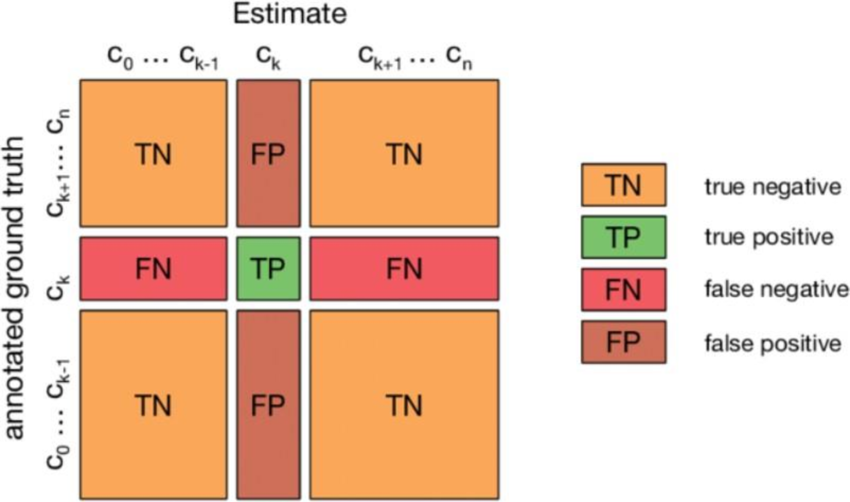
\includegraphics[width=100mm]{img/confusion-matrix.png}
	\caption{Martiz de confusión multiclase. Dada una predicción de una instancia de
		la clase $C_{k}$, la tabla muestra cuando se considera TP (verde), TN (naranja),
		FP (ocre) y FN (rojo). Fuente \cite{venkataramana2023}.}
	\label{fig:confusion-matrix}
\end{figure}

Estas clases son posteriormente empleadas para calcular diferentes métricas en
función de los requisitos que debe cumplir el modelo. Entre ellas, las más
empleadas son las siguientes:

\begin{itemize}
	\item \textbf{Exactitud o \textit{accuracy}}: Es el cociente entre el número de
	predicciones correctas y el total de predicciones realizadas. Se calcula
	como:
	\[
	\text{Exactitud}= \frac{TP + TN}{TP + TN + FP + FN}.
	\]
	
	\item \textbf{Precisión o \textit{precision}}: Es el cociente entre el número de
	verdaderos positivos y el total de predicciones positivas. Indica la
	exactitud de las predicciones positivas del modelo. Se calcula como:
	\[
	\text{Precisión}= \frac{TP}{TP + FP}.
	\]
	
	\item \textbf{Sensibilidad o \textit{recall}}: Es el cociente entre el número de
	verdaderos positivos y el total de casos reales positivos. Indica la
	capacidad del modelo para identificar todos los casos positivos. Se calcula como:
	\[
	\text{Sensibilidad}= \frac{TP}{TP + FN}
	\]
	
	\item \textbf{F1-Score}: Es la media armónica entre la precisión y la sensibilidad.
	Proporciona una única métrica que equilibra las dos anteriores y es
	especialmente útil cuando hay un desequilibrio entre las clases. Se calcula como:
	\[
	F1 = 2 \cdot \frac{\text{Precisión} \cdot \text{Sensibilidad}}{\text{Precisión}
		+ \text{Sensibilidad}}.
	\]
\end{itemize}

Por otra parte, se ha empleado la persistencia total como métrica para medir la
persistencia homológica de los datos en los distintos niveles de la red, además de
nuestra propuesta, la persistencia total normalizada.

\section{Proceso de entrenamiento}
\label{sec:train}

En esta etapa se ha optado por entrenar los modelos ResNet-18, DenseNet-121 y
EfficientNet-B0 bajo las siguientes condiciones para hacer un exhaustivo
análisis viendo cómo afectan a la topología de los datos y su rendimiento.

\begin{enumerate}
	\item \textbf{Optimización de Hiperparámetros:} Se realizó una búsqueda en
	rejilla (\textit{grid search}) para determinar los tamaños de lote óptimos (8,
	16, 32 y 64). Además, se emplearon los optimizadores Adam y SGD. Para Adam, se
	emplearon los hiperparámetros $\beta_{1} = 0.9$, $\beta_{2} = 0.999$ y
	$\varepsilon = 10^{-8}$.
	
	\item \textbf{Aumento de Datos:} Posteriormente, se aplicaron técnicas de aumento
	de datos al mejor modelo de cada familia identificado anteriormente. Las
	transformaciones incluyeron las descritas en la \autoref{sec:data-aug} para
	determinar las más beneficiosas en el contexto del entrenamiento final de
	los modelos, con el fin de mejorar su generalización.
	
	\item \textbf{Incorporación de Regularización Topológica:} Finalmente, se ha aplicado
	una búsqueda en rejilla al término $\alpha$ en el regularizador de dos formas.
	Se ha empleado $0, 0.001, 0.005, 0.01, 0.05, 0.1, 0.5$ y $1$ con los
	extractores de características de EfficientNet-B0 y DenseNet-121 congelados
	y para transferir DenseNet-121 de la especificidad Marca-Modelo a Marca. Estos
	mismos valores negados se han empleado para transferir EfficientNet-B0 de Marca
	a Marca-Modelo.
\end{enumerate}

Todas las tasas de aprendizaje fueron obtenidas a partir de una implementación realizada
del método propuesto por Leslie N. Smith
\cite{smith2017cyclicallearningratestraining}. Dicha técnica comienza aplicando una
tasa de aprendizaje muy baja que va aumentando exponencialmente en cada lote de entrenamiento
hasta un máximo establecido y registrando el error de entrenamiento asociado a cada
tasa. Finalmente, se determina el valor óptimo de la tasa escogiéndolo en algún punto
previo al mínimo donde la pendiente en la gráfica de error frente a tasa de aprendizaje
es más negativa. En particular, para la búsqueda se han empleado un mínimo de $10
^{-7}$ y un máximo de $1$. Las Tablas \ref{tab:bs-optim-marca} y
\ref{tab:bs-optim-marca-modelo} muestran las tasas de aprendizaje empleadas para
cada alternativa.

\begin{table}[H]
	\centering
	\begin{adjustbox}
		{max width=\textwidth}
		\begin{tabular}{|c|c|c|c|c|c|c|c|c|c|}
			\hline
			\textbf{Modelo}       & \multicolumn{4}{c|}{\textbf{SGD}} & \multicolumn{4}{c|}{\textbf{Adam}} \\
			\cline{2-9}           & \textbf{Lote 8}                   & \textbf{Lote 16}                  & \textbf{Lote 32} & \textbf{Lote 64} & \textbf{Lote 8} & \textbf{Lote 16} & \textbf{Lote 32} & \textbf{Lote 64} \\
			\hline
			\textbf{ResNet}       & 0.005                             & 0.001                             & 0.01             & 0.01             & 0.0005          & 0.001            & 0.001            & 0.001            \\
			\hline
			\textbf{DenseNet}     & 0.005                             & 0.01                              & 0.01             & 0.01             & 0.0005          & 0.001            & 0.001            & 0.001            \\
			\hline
			\textbf{EfficientNet} & 0.001                             & 0.05                              & 0.05             & 0.05             & 0.001           & 0.001            & 0.001            & 0.001            \\
			\hline
		\end{tabular}
	\end{adjustbox}
	\caption{Tasas de aprendizaje escogidas para los diferentes modelos, optimizadores
		y tamaños de lote en el conjunto de datos Marca.}
	\label{tab:bs-optim-marca}
\end{table}

\begin{table}[H]
	\centering
	\begin{adjustbox}
		{max width=\textwidth}
		\begin{tabular}{|c|c|c|c|c|c|c|c|c|c|}
			\hline
			\textbf{Modelo}       & \multicolumn{4}{c|}{\textbf{SGD}} & \multicolumn{4}{c|}{\textbf{Adam}} \\
			\cline{2-9}           & \textbf{Lote 8}                   & \textbf{Lote 16}                  & \textbf{Lote 32} & \textbf{Lote 64} & \textbf{Lote 8} & \textbf{Lote 16} & \textbf{Lote 32} & \textbf{Lote 64} \\
			\hline
			\textbf{ResNet}       & 0.005                             & 0.01                              & 0.01             & 0.05             & 0.0005          & 0.001            & 0.001            & 0.001            \\
			\hline
			\textbf{DenseNet}     & 0.005                             & 0.01                              & 0.01             & 0.01             & 0.0005          & 0.001            & 0.001            & 0.005            \\
			\hline
			\textbf{EfficientNet} & 0.05                              & 0.05                              & 0.05             & 0.05             & 0.001           & 0.005            & 0.005            & 0.005            \\
			\hline
		\end{tabular}
	\end{adjustbox}
	\caption{Tasas de aprendizaje escogidas para los diferentes modelos, optimizadores
		y tamaños de lote en el conjunto de datos Marca-Modelo.}
	\label{tab:bs-optim-marca-modelo}
\end{table}

Se ha empleado \textit{early stopping} como criterio de parada con una paciencia
de $5$ épocas respecto a los valores de pérdida del conjunto de validación.
Todos los modelos han sido entrenados sobre los conjuntos de datos de Marca y
Marca-Modelo.

\section{Visualización de la homología persistente}

Para cada una de las redes entrenadas y seleccionadas en la \autoref{sec:train},
hemos medido la persistencia de las clases de homología de dimensión 0 y 1
respecto a los conjuntos de datos de entrenamiento, validación y test. En un
inicio, se valoró estudiar la topología respecto al conjunto de entrenamiento al
completo. Debido al gran coste en memoria que suponía, finalmente se optó por evaluarla
para un subconjunto escogido de manera aleatoria de los datos de entrenamiento con
el mismo número de instancias que los conjuntos de validación y test.

%La visualización de los datos a través de la red se ha realizado mediante el uso de un algoritmo de reducción no lineal de la dimensionalidad conocido como \textbf{incrustación lineal local} o \textbf{\textit{locally lineal embedding}} (LLE). Este método consiste en describir cada instancia del conjunto en coordenadas de sus $k$ vecinos más cercanos, siendo $k \in \N$ la dimensionalidad de la nueva representación. Como dichos vecinos no tienen por qué formar una base, las coordenadas se escogen de manera que la combinación lineal realizada minimice el error cuadrático medio respecto a las coordenadas originales.

Para la visualización de la homología persistente se han empleado gráficas que
muestran la persistencia total y la persistencia total normalizada en función
del instante de avance de los datos en la red. Además, se ha utilizado el código
de barras descrito en la \autoref{sec:barcode} para ofrecer un mayor detalle en
ciertos momentos del estudio.

Por último, se ha empleado el método Grad-CAM \cite{Selvaraju_2019} para visualizar
la intensidad de las activaciones mediante un mapa de calor sobre las imágenes originales.

\endinput
%--------------------------------------------------------------------
% FIN DEL CAPÍTULO.
%--------------------------------------------------------------------